\chapter{Množice}

\section{In še množice}

Zadnji izmed vgrajenih podatkovnih tipov, ki si ga moramo pogledati, so množice. Množice za predstavitev podatkov uporabljamo takrat, ko želimo, da posamezen podatek obravnavamo največ enkrat. Ker nam Python poleg tega nad množicami omogoča izvedbo osnovnih operacij, kot so unija, presek in razlika, množice zelo spominjajo na matematične množice. 

\section{Uporaba množic}

Množice podobno kot slovarje zapisujemo v zavite oklepaje, znotraj katerih naštejemo elemente. Množico elementov 1, 2 in 3, bi torej naredili takole:
\begin{lstlisting}[language=Python]
>>> mnozica = {1,2,3}
>>> mnozica
{1, 2, 3}
>>> type(mnozica)
<class 'set'>
\end{lstlisting}
Kljub temu, da množice uporabljajo podoben zapis kot slovarji, ju Python med seboj brez problemov loči, saj slovarji za razliko od množic vsebujejo pare ključ: vrednost. Do težave pride le takrat, ko je množica oziroma slovar prazen. Do praznega slovarja pridemo tako, da podamo zavite oklepaje brez elementov:
\begin{lstlisting}[language=Python]
>>> slovar = {}
>>> slovar
{}
>>> type(slovar)
<class 'dict'>
\end{lstlisting}
Do prazne množice pridemo z uporabo funkcije \texttt{set}, ki jo pokličemo brez argumentov:
\begin{lstlisting}[language=Python]
>>> mnozica = set()
>>> mnozica
set()
>>> type(mnozica)
<class 'set'>
\end{lstlisting}

\section{Omejitve pri uporabi množic}

Elementi množic imajo zelo podobne omejitve kot ključi slovarji, za katere prav tako velja, da lahko posamezno vrednost vsebujejo največ enkrat. Prav tako kot za ključe slovarjev tudi za množice velja, da lahko vsebujejo le nespremenljive podatkovne tipe. 

Množice predstavljajo neurejeno strukturo, kar pomeni, da vrstni red elementov množice ni pomemben in tudi ni določen. Elementi torej niso vezani na indekse, zato množic ne moremo indeksirati in nad njimi delati rezine:
\begin{lstlisting}[language=Python]
>>> mnozica = {1,2,3}
>>> mnozica[0]
TypeError: 'set' object is not subscriptable
\end{lstlisting}
Prav tako nad množicami ne moremo izvajati aritmetičnih operacij, kot smo jih npr. lahko izvajali nad nizi:
\begin{lstlisting}[language=Python]
>>> {1,2,3}*3
TypeError: unsupported operand type(s) for *: 'set' and 'int'
>>> {1,2,3} + {4,5,6}
TypeError: unsupported operand type(s) for +: 'set' and 'set'
\end{lstlisting}

\section{Osnovne operacije nad množicami}

Kaj pa pravzaprav potem z množicami sploh lahko počnemo. Ko množico enkrat imamo se lahko čez njo sprehajamo z zanko \texttt{for}:
\begin{lstlisting}[language=Python]
>>> mnozica = {1,2,3}
>>> for element in mnozica:
	print(element)
1
2
3
\end{lstlisting} 
Poleg tega lahko preverjamo ali množica določen element vsebuje (ali ne) z operatorjema vsebovanosti:
\begin{lstlisting}[language=Python]
>>> mnozica = {1,2,3}
>>> 1 in mnozica
True
>>> 2 not in mnozica
False
>>> 4 in mnozica
False
\end{lstlisting}

Številu elementov v množici pravimo tudi moč množice, do katere pridemo enostavno s klicem vgrajene funkcije \texttt{len}
\begin{lstlisting}[language=Python]
>>> len({1,2,3})
3
\end{lstlisting}

\begin{zgled}
Napiši funkcijo \texttt{razlicni}, ki kot argument sprejme niz, kot rezultat pa vrne število različnih znakov, ki v nizu nastopajo
\end{zgled}
\begin{resitev}
Najprej bomo niz pretvorili v množico s funkcijo \texttt{set}. Ker množica posamezen element vsebuje največ enkrat, se bomo s tem znebili vseh potencialnih ponovitev znakov. Potem samo še izračunamo in vrnemo moč množice.
\begin{lstlisting}[language=Python,numbers=left]
def razlicni(niz):
    mnozica = set(niz) # odstranitev duplikatov
    return len(mnozica) # moc mnozice
\end{lstlisting}
\end{resitev}

Tudi primerjalni operatorji so zdaj prilagojeni matematični interpretaciji množic. Ali je prva množica podmnožica druge, lahko npr. ugotovimo z operatorjem \texttt{<=}:
\begin{lstlisting}[language=Python]
>>> {1,2,3} <= {1,2,3,4}
True
\end{lstlisting}

\section{Presek, unija in razlika}

Primeri najbolj tipičnih operacij, ki jih prikazujejo diagrami na sliki \ref{img:mnozice}, so seveda presek (\texttt{A \& B}), unija (\texttt{A | B}) in razlika (\texttt{A - B}).
\begin{figure}
    \centering
    \begin{tabular}{cc}
    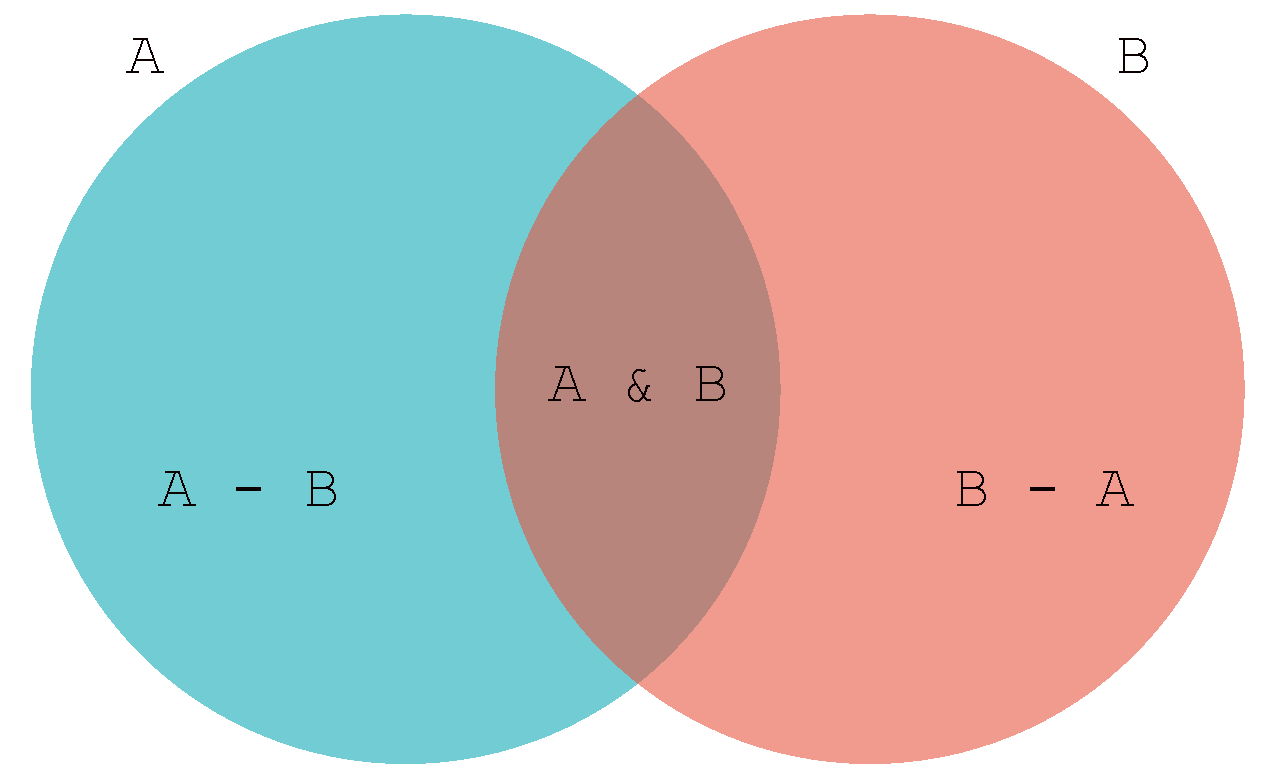
\includegraphics[width=0.45\linewidth]{img/mnozice1.pdf} & 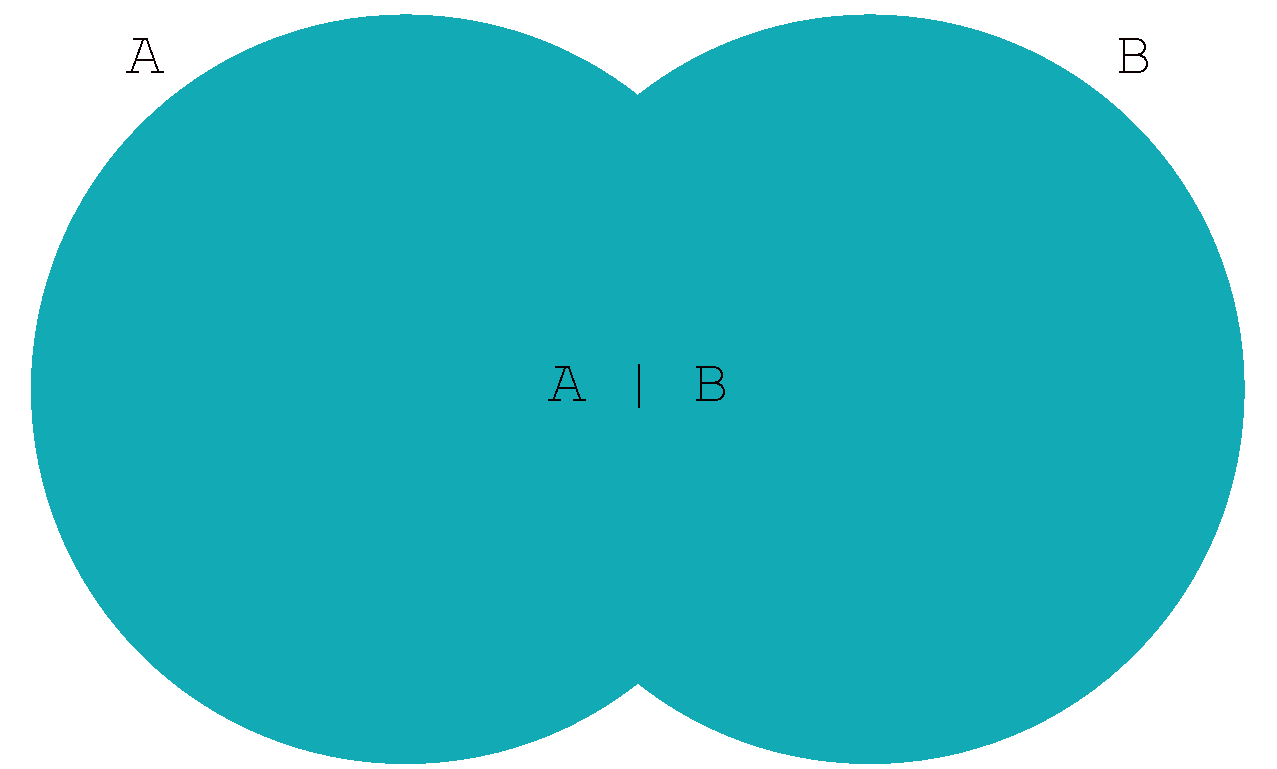
\includegraphics[width=0.45\linewidth]{img/mnozice2.pdf}\\
    \end{tabular}
    \caption{Vennova diagrama, ki ponazarjata osnovne operacije nad množicami. Slika na levi prikazuje razliko (\texttt{A-B} in \texttt{B-A}) in presek (\texttt{A \& B}) med množicama \texttt{A} in \texttt{B}. Slika na desni prikazuje unijo (\texttt{A | B}) med množicama \texttt{A} in \texttt{B}}
    \label{img:mnozice}
\end{figure}
Primer uporabe gornjih operacij je sledeč:
\begin{lstlisting}[language=Python]
>>> {1,2,3} & {3,4,5} # presek
{3}
>>> {1,2,3} | {3,4,5} # unija
{1,2,4,5}
>>> {1,2,3} - {3,4,5} # razlika
{1,2}
\end{lstlisting}

\section{Zgled uporabe množic}
Ker so bili sprotni zgledi v tem poglavju relativno skopi, bomo to nadoknadili z malo daljšim zgledom, s katerim bomo povadili tudi slovarje in mogoče še kaj. 
